\documentclass[11pt,a4paper,twocolumn]{article}
\usepackage[utf8]{inputenc}
\usepackage{amsmath}
\usepackage{amsfonts}
\usepackage{amssymb}
\usepackage{hyperref}
\usepackage{graphicx}
\usepackage{tikz}
\usepackage[justification=centering]{caption}
\usepackage{subcaption}
\usepackage[left=1in,right=1in,top=1in,bottom=1in]{geometry}
\author{Daniel Deutsch and Dan Crankshaw}
\title{Machine Learning: Final Paper}
\date{}
\begin{document}
\maketitle

\section{Introduction}

A common problem in the field of machine learning is correctly identifying
handwritten words. The applications of
such a model are clear, and have already been implemented in situations like
the US postal service to sort mail based on the zip code.

The idea behind our approach is to compare how well two algorithms perform in
completing the optical character recognition task. The first algorithm is an
artifical neural network that will try to classify characters based on
their pixel values. The second algorithm is a combination of the previous
neural network and a hidden markov model, which will take into account the
probability of specific letter combinations. We hope that the addition of contextual
about the surrounding letters will help improve the accuracy of the neural
network.

\section{Related Work}

Feng et al.\cite{feng2008hidden} explores this idea of combining classification with a sequence
model in order to perform handwriting recognition on a large vocabulary corpus. They used a
joint-boosting algorithm to not only identify the letters, but perform letter segemenation. They
combined information about each individual letter with knowledge of the context of the letter in the
form of a supervised HMM.

Although the approach they take is more complicated, including the use of an emsemble of HMMs and
many more features, their success indicates that the combination of classification with an HMM is a
viable approach for the handwriting recognition problem.

\section{The Algorithms and Data}

\subsection*{Data}

The data that will be used in the training and evaluation of the ANN and the HMM was gathered from
\href{http://ai.stanford.edu/~btaskar/ocr/}{an optical character recognition dataset from
Stanford University}.
The data is a collection of handwritten letters segemented from words in which all uppercase
characters have been removed. We took the raw data and removed specific features included in the
data that we intended not to use. The resulting data set is a list of binary pixel values of each
character's 16 by 8 image.  \begin{figure}[h]
    \centering
    \includegraphics{img/ml.jpg}
    \includegraphics{img/alphabet.jpg}
    \caption{An example of the data set}
\end{figure}

The data can often be difficult to read for a human as Figure 1 demonstrates.
Although it is possible to make out each letter, this task is made much
easier by looking at the context of the word and anticipating what the letter
should be. The figure also illustrates that many of the same letters are a
variety of different sizes and are placed at different locations within the
image. The quality of the data may make it difficult for the ANN to learn how
to recognize each letter. However, the combination of the ANN and the HMM may
be a good simulation of how a human would approach the problem: try to
recognize the letter, then use context clues to figure out which character it
is.

The corpus used to learn the transmission probabilities for the HMM is a
a Project Gutenberg plain-text copy of \emph{Moby Dick}. We cleaned the
corpus by converting all letters to lowercase and removing all non-alphabetic
characters (i.e.\ numbers and punctuation). Our training corpus is the first
half of the text and the test corpus is the second half of the text.

\subsection*{The Algorithms}

The two algorithms that we intend to use to accomplish the character recognition goal are an
artificial neural network (ANN) and a hidden markov model (HMM). The idea is to compare the accuracy
of the ANN to a combination of both the ANN and HMM to see if adding knowledge of word context to
the model increases accuracy on the datasets.

\subsubsection*{Neural Network Theory}

The original idea behind the artifical neural network was to simulate connections between neurons in
the brain. Each neuron receives a message, performs some type of computation, and sends a new
message to the neurons to which it is connected. For the artificial neural network, the intial input
is derived from the features of a data point. Based on this input, each neuron computes an
activation function (typically the sigmoid function) to see if it should be on or off. The new
values that are computed are multipled by a transition weight to the next layer of neurons. This
process repeates until the output layer has been reached. The values of each output neuron represent
a likelihood that the input data is of a specific class.

In order to train the algorithm, the backpropagation algorithm assigns specific error values to each
individual node, which creates the gradient function based on each of the parameters. With the
gradient function, an optimization algorithm like gradient descent can be use to find an optimum
value for each parameter. Neural networks are not convex, so there is no guarantee that the solution
is the global optimum.

\begin{figure}[h]
\centering
\caption{An example neural network}
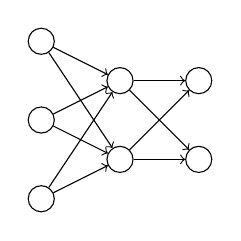
\begin{tikzpicture}

\node (x1) at (0, 0) [draw,shape=circle]{};
\node (x2) at (0, 1) [draw,shape=circle]{};
\node (x3) at (0, 2) [draw,shape=circle]{};

\node (x4) at (1, 1.5) [draw,shape=circle]{};
\node (x5) at (1, 0.5) [draw,shape=circle]{};

\node (x6) at (2, 1.5) [draw,shape=circle]{};
\node (x7) at (2, 0.5) [draw,shape=circle]{};

\draw [->] (x1) -- (x4);
\draw [->] (x2) -- (x4);
\draw [->] (x3) -- (x4);

\draw [->] (x1) -- (x5);
\draw [->] (x2) -- (x5);
\draw [->] (x3) -- (x5);

\draw [->] (x4) -- (x6);
\draw [->] (x5) -- (x6);

\draw [->] (x4) -- (x7);
\draw [->] (x5) -- (x7);

\end{tikzpicture}
\end{figure}

In Figure 2, each neuron is represented with a circle. Each weight parameter that is learned by the
backpropagation algorithm is shown by a line that connects the neurons in each layer.

\subsubsection*{Neural Network Implementation}

The ANN will be trained on the pixel values for each letter image. Each training example is a 16 by
8 pixel image which amounts to an input size of 128. In order to help improve the accuracy of the
classifier, we included a bias term on the input and hidden layers. Therefore, the input size for
the ANN is 129 nodes.

Similarly, since we are trying to classify each image as a letter, there will need to be 26 output
nodes, one for each lowercase letter in the alphabet. Therefore, the input and output sizes are set.
The only parameters left to tune for the ANN are the number of hidden layers and the number of nodes
within each hidden layer.

In order to find the best values for these parameters, we ran a series of tests on the development
data set to try and tune the parameters. We compared the accuracies of each model on the development
dataset to try and find the optimal parameters.

The following was generated by randomly initializing an ANN with the given hidden layer sizes, then
training them all on the same data. This process is repeated 20 times per data point, and the
average accuracy is given. The accuracy is determined by if the classifier gets the data point
exactly correct. Another common metric is to test if it got the right answer within the top 5
guesses, but that is not used here.

For the ANN with one hidden layer, the only parameter than can be changed is the number of hidden nodes in that layer.

\begin{figure}[h]
    \caption{Accuracies of two-layer networks}
    \centering
    \begin{tabular}{|c|c|}
        \hline 
        Hidden Nodes & Accuracy \\ 
        \hline 
        25 & 54.86\% \\ 
        \hline 
        50 & 54.24\% \\ 
        \hline 
        75 & 52.13\% \\ 
        \hline 
    \end{tabular} 
\end{figure}

Since all three data points are relatively similar, and the smaller neural
network will train faster, we will use a network with one hidden layer and 25 nodes
in that layer.

This data is indicative of our belief that the neural network might have some
difficultly classifying this dataset. The input seems to be a relatively
difficult dataset with some noise. Since adding more nodes to the hidden layer
did not imporve the accuracy significantly enough, it's evident that the
network is having a hard time learning the data. It may have reached its
maximal ability to learn. We hope that the combination of the HMM with the ANN
will help improve these accuracies.

One other idea that we tried was to add a second hidden layer to see if
increasing the number of weights allowed for improvement. With a small number
of tests, the amount of improvement was almost non-existent. Therefore, given
the extra amount of time it takes to train a neural network with two hidden
layers, we concluded that it was not worth the investment.

Therefore, the neural network that we will use in our experiments in
combination with and against the HMM will be a neural network with 128 input
nodes, 25 hidden nodes, and 26 output nodes, not counting the bias units.

Since it is possible to describe a neural network as a series of matrix multiplications, its
implementation will involve some non-trivial linear algebra functions. In order to do this
effectively in Java, we use the \href{http://math.nist.gov/javanumerics/jama/}{Java Matrix Package}.


\subsubsection*{Hidden Markov Model Theory}


\subsubsection*{Hidden Markov Model Implementation}

We trained the HMM in a supervised setting, directly learning the parameters
from labeled data. We treat the actual letters that make up a word as the
hidden nodes ($z_i$) and the letters predicted by the ANN based on that
input as the observed nodes ($x_i$). The first set of parameters that the HMM
needs to learn are the emission probabilities $P(x_i | z_j)$. This is the probability
that the ANN predicts an observed letter $x_i$ given a letter representing
the state $z_j$. We learn these probabilities 

ADD DISCUSSION OF THEORY BEHIND HMM
ADD NOTE ABOUT LEARNING EMISSION PROBS BAYESIAN VS NON BAYESIAN


\section{Results}

In order to compare the implementation and accuracy of the ANN versus the HMM-ANN combination, we
compared their performances with three different metrics: the percentage of letters correct, the
percentage of fully correct words, and the average percentage of letters correct per word.

In the following figures, we compare the two algorithms with each of the three accuracy metrics. The
neural network was not retrained between tests. Its results were used to calculate the emission
probabilities for the HMM\. The HMM, however, was retrained with four different subsets of the
training corpus: the first 12.5\% of the corpus, the first 25\%, the first 50\%, and then all of the
training data. Each algorithm was then tested on a random 10\% of the same test dataset, and the
results were averaged. This process was repeated on three subsets of words: small (2-4 letters),
medium (5-8 letters), and large (9+ letters) words.

\begin{figure}[h]
\centering
\caption{Percentage of letters correct}
\includegraphics[scale=0.55]{img/lettersCorrect.png}
\end{figure}

\begin{figure}[h]
\centering
\caption{Percentage of fully correct words}
\includegraphics[scale=0.55]{img/wordsCorrect.png}
\end{figure}

\begin{figure}[h]
\centering
\caption{Average percentage of letters correct per word}
\includegraphics[scale=0.55]{img/wordCorrectness.png}
\end{figure}


\section{Analysis}

We hypothesized that increasing the size of the training corpus would increase the accuracy of the
HMM because in order for the transmission probabilities to converge, we would need to look at a
certain amount of data. However, there was no significant difference in the HMM accuracy as we
changed the size of the training corpus. It is possible that even the smallest corpus was already
large enough for the transmission probabilites to have converged at approximately 14,000 words.

From Figures 4 and 5, it is evident that as the length of the word increases, the accuracy of the
ANN-HMM combination decreases. We hypothesize that once the HMM begins to incorrectly identify a
sequence, it tends to continue to do so because of the weight of the transmission probabilities on
predicting the most probable sequence. In order to get a sequence back on the right track, we would
need a high correct emission probability and a high probability of transitioning from the previous
incorrect letter to the current correct letter, which effectively breaks the reasons behind using a
HMM\. Because we use the same ANN-HMM combination on our short and long word predictions, we assume
the same probability of getting a starting down an incorrect subsequence at a given position in a
word regardless of the length of the word. Because the longer words have more positions at which to
start down a wrong sequence, and will tend to have more letters remaining in the word to be wrongly
predicted once an incorrect subsequence is started down, longer words will tend to have more
incorrect letters. *****However, this is still a hypothesis and we would need to run more
experiments to verify this.

One interesting trend that we did not expect to see in the data is the slight increase in accuracy
of the ANN on the data set as the word length increases. This was surprising because the ANN
predicts each letter independently, so changing how the letters are grouped into words should not
have affected the accuracy. One potential explanation is that the ANN is much better at classifying
some letters than others. If the longer words tend to contain higher concentrations of those
``eaiser'' letters, then the ANN would have a higher accuracy on the larger word bucket. 

In order to investigate this further, we looked at the accuracy of the ANN on each specific letter.
As you can see from Figure 7, the results are highly variable, and there are even several letters
that have 0\% accuracy.

\begin{figure}[h]
\centering
\caption{Individual letter accuracies for the ANN}
\includegraphics[scale=0.55]{img/letterPercentages.png}
\end{figure} 

One potential reason for this high variability is that the number of training examples for the
different letters varies by an order of magnitude. The letters on which we did predicted very poorly
tend to occur less often in English, and therefore we did not have as many training examples for
those letters. This does not prove that the longer words contain less of the harder letters, but it
supports that it is a valid hypothesis. 


\section{Conclusion}

While our models did significantly better than random guessing, we still expected higher accuraices
that what we were able to obtain. It seems that the root of our issues with the HMM are directly
tied to the low accuracies of the neural network. We believe a lot of the issues with the neural
network were based on what turned out to be a very noisy and relatively sparse data set. 

One step in trying to improve the model would be to use less noisy data. We could perform optical
character recognition on typed letters instead of handwritten ones as this would minimize the amount
of variation between each letter. 

Another option would be to add more features to the data set other than just the character's pixel
values. We could consult the computer vision literature to help with this additional feature
engineering. 


\bibliography{refs.bib}
\bibliographystyle{plain}

\end{document}
